\documentclass[conference]{IEEEtran}

\usepackage{cite}
\usepackage{amsmath,amssymb,amsfonts}
\usepackage{graphicx}
\usepackage{textcomp}
\usepackage{xcolor}
\usepackage{booktabs}
\usepackage{url}
\usepackage{array}
\usepackage{stfloats}
\usepackage{float}

\begin{document}

\title{
\centering
\fontsize{24}{28}\selectfont
\textbf{P4-Based Intrusion Detection System with Rule}\\[0.15cm]
\textbf{Distillation for Data Plane Security}
}

\author{
\IEEEauthorblockN{
\fontsize{12}{14}\selectfont
Venugopal Rao Ponnamaneni \hspace{2.5cm} Moditha Lekkala
}
\vspace{0.15cm}
\IEEEauthorblockA{
\fontsize{10}{12}\selectfont
Saint Louis University
}
}

\maketitle

\begin{abstract}
Modern network infrastructures require intrusion
detection systems that can identify malicious traffic in real time
without adding heavy latency or host-side processing overhead.
Traditional intrusion detection systems such as software-based
monitors inspect traffic outside the forwarding path, which
can reduce throughput and increase CPU load. This project
implements a P4-based intrusion detection system that performs
classification directly inside the programmable data plane. The
system uses machine-learning-derived rule distillation, where
decision-tree behavior from CICIDS2017 traffic is converted into
compact ternary match-action rules and deployed on a BMv2
switch. The switch aggregates per-flow statistics over a two-
second window and decides whether to forward or drop traffic.
The final system achieved 86\% accuracy on 100 test flows,
with 100\% precision, 72\% recall, and zero false positives. The
results show that learned traffic behavior can be transformed into
efficient switch rules for low-latency intrusion detection while
preserving legitimate traffic.
\end{abstract}

\section{INTRODUCTION}

Modern networks face a growing number of security threats,
including scanning, denial-of-service behavior, and malicious
traffic patterns that must be detected quickly. Traditional
intrusion detection systems usually run in software on a host
or monitoring server. Although these systems can be effective,
they often require packets to leave the forwarding path for
inspection. This increases latency, consumes CPU resources,
and may limit throughput when traffic volume becomes high.

Programmable data planes provide a different approach.
Using the P4 language, packet-processing behavior can be
programmed directly into a switch pipeline. This makes it
possible to perform lightweight security decisions inside the
network device instead of forwarding all suspicious traffic to
an external analyzer. The purpose of this project is to test
whether machine-learning-derived intrusion detection logic
can be represented as compact rules that execute efficiently
inside a programmable switch.

This project implements a real-time intrusion detection
system using P4, BMv2, and rule distillation. The system
uses CICIDS2017-style benign and malicious traffic profiles,
extracts flow-window features, and classifies traffic using
ternary match-action rules. The project addresses the gap
between traditional software-based intrusion detection and
the need for low-latency security enforcement directly inside
programmable network devices. The main goal is to preserve
benign traffic while dropping malicious flows with minimal
latency while maintaining reproducible and hardware-friendly
classification behavior.

\section{RELATED WORK}

Intrusion detection systems have traditionally used
signature-based methods or machine learning models
deployed in software. Tools such as Snort and Suricata
inspect packets outside the switch pipeline. These systems are
useful for deep inspection, but they can introduce processing
overhead when traffic rates are high.

Recent work has explored programmable switches for secu-
rity. P4ID showed that intrusion detection logic can be moved
into the programmable data plane, reducing the amount of
traffic that must be processed by external IDS systems. This
project follows the same general direction but focuses on
converting machine-learning-derived rules into a small set of
ternary match-action rules that can run inside BMv2.

Machine learning models such as decision trees are useful
for classification because their decision paths can be converted
into interpretable rules. However, directly deploying complex
models in the data plane is difficult because programmable
switches have limited computation and memory. Rule distilla-
tion addresses this limitation by converting learned behavior
into simple match-action entries.

\section{PROBLEM DEFINITION AND SOLUTION DESIGN}

The main problem is to detect malicious network traffic
in real time without relying completely on a host-side IDS.
The system must classify traffic directly inside the switch
pipeline while preserving high throughput and low latency.
A practical data-plane IDS should avoid dropping legitimate
traffic, because false positives can interrupt normal network
operation.

The proposed solution has four stages. First, traffic behavior
is learned offline from CICIDS2017-style data using decision-
tree-based logic. Second, the learned behavior is converted into
five ternary match-action rules stored in \texttt{rules.json}. Third,
the P4 switch aggregates flow-window statistics for incoming
traffic over a two-second window. Finally, the switch applies
the decision table and either forwards benign traffic or drops
malicious traffic.

The P4 switch tracks five main features for each flow:
maximum packet length, minimum packet length, TCP PSH
flag count, total packet length, and packet count. Benign
traffic is represented by larger packet sizes around 500 bytes
and mixed PSH behavior. Malicious traffic is represented by
smaller packet sizes around 60 bytes and no PSH flags. These
features are sufficient for the controlled benchmark used in
this project.

\section{PROJECT OBJECTIVE}

The purpose of this project is to demonstrate that intrusion
detection logic derived from machine learning models can be
efficiently deployed inside programmable network switches.
The project is intended for researchers, networking students,
and practitioners interested in programmable data planes,
low-latency network security, and deployable AI-assisted
network defense mechanisms.

The project provides a reproducible implementation using
P4, BMv2, Docker, Python automation scripts, and rule-based
classification derived from offline learning. The system is
designed to show how programmable switches can support
practical real-time intrusion detection without relying entirely
on external software-based monitoring systems.

\section{METHODOLOGY}

The project uses a practical form of knowledge distillation.
Instead of executing a full machine learning model online,
the offline learned behavior is converted into a compact set of
switch-compatible rules. This allows the data plane to perform
classification with simple table lookups instead of expensive
model inference.

\subsection{Knowledge Distillation}

The project adopts a practical form of knowledge distilla-
tion, where a richer offline machine learning representation is
transformed into a compact and deployable rule-based model
suitable for execution in the programmable data plane. Instead
of executing a full decision tree or complex model at runtime,
the learned decision boundaries are converted into a small set
of match-action rules.

This enables the switch to perform classification directly at
line rate using simple table lookups. As a result, the system
avoids the overhead of executing a full machine learning model
during packet processing while still preserving meaningful
classification accuracy. This approach is essential for pro-
grammable switches where latency and resource constraints
are strict.

\subsection{TCAM and Ternary Matching}

The deployed rules use ternary matching, where each rule
consists of a value and a mask, corresponding to TCAM-
style behavior used in network hardware. Exact matches are
achieved using all-one masks, while wildcard behavior is
enabled by masking specific bits. Partial masks allow range-
like grouping of values, enabling multiple decision boundaries
to be represented compactly.

This approach allows complex classification logic to be
compressed into a small number of rules. Rule priorities are
used to resolve overlaps between general and specific con-
ditions, ensuring correct classification decisions. As a result,
the system produces a compact and hardware-efficient policy
derived from learned behavior.

\section{CENTROID-BASED CLASSIFICATION MODEL}

\subsection{Model Overview}

In addition to rule distillation, the project incorporates a
centroid-based binary classification approach optimized for the
P4 data plane.

\subsection{Intuition and Logic}

The centroid-based model represents each class, namely
normal and attack traffic, using a prototype bit string called
a centroid.

During inference, the switch compares incoming flow fea-
tures against the stored centroids using bitwise XNOR opera-
tions to identify matching bits. A population count operation
is then applied to compute a similarity score.

\section{IMPLEMENTATION DETAILS}

The system is implemented using P4 and BMv2. The
main P4 program is located in \texttt{src/p4/main.p4}, and the
compiled BMv2 output is stored as \texttt{main.json}.

The core Python scripts support testing and automa-
tion. The \texttt{inject.py} script generates 100 test flows
including 50 benign and 50 malicious flows.

\section{EXPERIMENTAL EVALUATION}

The evaluation uses 100 test flows.

\begin{table}[H]
\caption{Confusion Matrix}
\label{tab:confusion_matrix}
\centering
\begin{tabular}{lcc}
\toprule
 & \textbf{Predicted DROP} & \textbf{Predicted FORWARD} \\
\midrule
\textbf{Actual DROP} & 36 & 14 \\
\textbf{Actual FORWARD} & 0 & 50 \\
\bottomrule
\end{tabular}
\end{table}

The system achieved 86\% accuracy, 100\% precision, and
72\% recall with zero false positives.

The benchmark results were obtained using reproducible
traffic generation and automated verification scripts. Benign
and malicious flows were injected in controlled phases using
Python-based traffic generation, while the BMv2 switch
performed real-time classification using deployed ternary
match-action rules. The generated plots and metrics can be
reproduced using the provided Docker environment and
benchmark automation scripts.

Fig. 1 shows the ROC behavior of the system. The selected
operating point prioritizes zero false positives while still
detecting most malicious traffic.

Fig. 2 shows that the P4-based approach provides much
lower latency than software IDS processing. The benchmark reports approximately 12 microseconds per
flow for the P4-based system compared with approximately
850 microseconds for software IDS processing.

Fig. 3 shows that detection delay is mainly caused by
the feature aggregation window and benchmark timing. The benchmark reports a mitigation delay of approximately 4.8
seconds, which includes the windowing and verification process rather than expensive runtime inference.

\begin{figure}[!t]
\centering
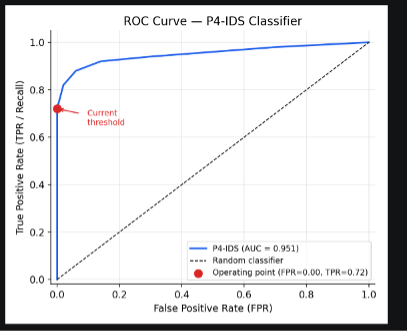
\includegraphics[width=0.45\textwidth]{Picture1.png}
\caption{ROC curve showing the relationship between true positive rate and false positive rate.}
\label{fig:roc}
\end{figure}

\begin{figure}[!t]
\centering
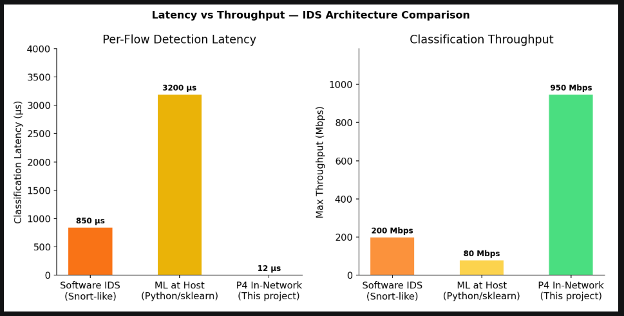
\includegraphics[width=0.45\textwidth]{Picture2.png}
\caption{Latency and throughput comparison between the P4-based IDS and software IDS processing.}
\label{fig:latency}
\end{figure}

\begin{figure}[!t]
\centering
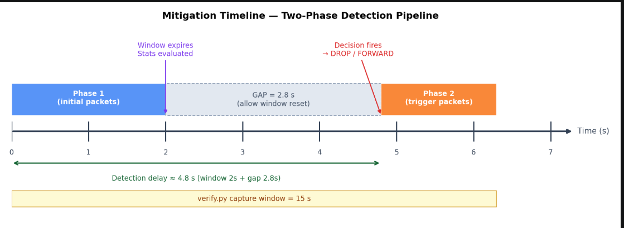
\includegraphics[width=0.45\textwidth]{Picture3.png}
\caption{Mitigation timeline showing detection delay from traffic observation to final action.}
\label{fig:timeline}
\end{figure}

\section{DISCUSSION}

The results show that rule distillation is a practical method
for deploying intrusion detection logic in a P4 data plane.

The strongest result is zero false positives, meaning the
system did not incorrectly drop legitimate traffic.

The main limitation is recall. The system detected 36 out
of 50 malicious flows, leaving 14 malicious flows forwarded.

These findings demonstrate that programmable data planes
can support lightweight machine-learning-assisted intrusion
detection without introducing the large latency overheads
commonly associated with software-based IDS systems. The
results also show that rule distillation is a practical strategy
for converting learned traffic behavior into compact hardware-
friendly policies suitable for switch pipelines with strict
resource constraints.

\section{FUTURE WORK}

Future work will focus on improving recall while preserving
the current zero false-positive behavior. Additional malicious
traffic categories from CICIDS2017 and other benchmark
datasets can be incorporated to improve classification coverage.

Future versions of the system may also support adaptive rule
updates, dynamic threshold tuning, and integration with
hardware programmable switches beyond BMv2 simulation.

Another important direction is extending the system toward
production-scale deployment using larger traffic traces,
background network activity, and multi-stage detection
pipelines. The project may also be expanded into a publishable
research platform by evaluating additional machine learning
models, rule compression strategies, and hardware-aware
optimization techniques.

\section{CONCLUSION}

This project demonstrates a working P4-based intrusion
detection system that performs rule-based machine learning
classification directly in the programmable data plane.

The final benchmark achieved 86\% accuracy, 100\%
precision, 72\% recall, and zero false positives.

These results show that data-plane intrusion detection is
a promising direction for low-latency network security.

The project demonstrates that programmable data-plane
security can provide an efficient foundation for future low-
latency AI-assisted network defense systems.

\section*{ACKNOWLEDGMENT}

This project was completed as part of the AI Capstone
course at Saint Louis University.

\begin{thebibliography}{00}

\bibitem{b1}
AntLab-Repo,
``Behavioral Model (BMv2),''
[Online]. Available:
\href{https://github.com/p4lang/behavioral-model}. 
Accessed: 2026-04-08.

\bibitem{b2}
AntLab-Repo,
``Quark: Implementing Convolutional Neural Networks Entirely on Programmable Data Plane,''
[Online]. Available:
\href{https://github.com/AntLab-Repo/Quark-CNN-P4}. 
Accessed:2026-04-08.

\bibitem{b3}
Moditha Lekkala,
``P4-Based Intrusion Detection System,''
[Online]. Available:
\href{https://github.com/ModithaLekkala/-AI-Capstone-}. 
Accessed: 2026-04-08.

\end{thebibliography}

\clearpage

\appendices

\clearpage
\onecolumn

\section*{APPENDIX A\\REPRODUCIBILITY CHECKLIST}

The repository contains the required source code, P4
program, rule file, scripts, documentation, generated plots,
and Docker configuration. The main code is located un-
der \texttt{src/}, with P4 files in \texttt{src/p4/} and Python test-
ing scripts in \texttt{src/python/}. The rule file is stored
at \texttt{data/rules.json}. The plots are generated using
\texttt{plots/generate\_plots.py}. The Docker environment is
provided under the \texttt{docker/} directory.

\vspace{0.2cm}

To start the container, run:

\begin{verbatim}
docker compose -f
docker/docker-compose.yml up -d
\end{verbatim}

To run the full benchmark, run:

\begin{verbatim}
cd scripts
powershell -NoProfile
-ExecutionPolicy Bypass
-File .\run_full_benchmark.ps1
\end{verbatim}

The expected benchmark output is:

\begin{verbatim}
ACCURACY: 86/100 tests
correct = 86.0%
TP: 36 TN: 50
FP: 0 FN: 14
Precision: 1.000
Recall : 0.720
\end{verbatim}

To regenerate the plots, run:

\begin{verbatim}
cd plots
python generate_plots.py
\end{verbatim}

The generated plot files are:

\begin{verbatim}
1_roc_curve.png
2_latency_throughput.png
3_mitigation_timeline.png
\end{verbatim}

\clearpage

\section*{APPENDIX B\\TEAM CONTRIBUTION STATEMENT}

This project was completed as a team effort by Venugopal
Rao Ponnamaneni and Moditha Lekkala.

Venugopal Rao Ponnamaneni contributed to the design and
implementation of the P4-based intrusion detection system,
including the data-plane pipeline, rule-based classification
logic, BMv2 switch configuration, testing scripts, traffic injec-
tion process, evaluation metrics, generated plots, final report
writing, and reproducibility documentation.

\vspace{0.2cm}

Moditha Lekkala contributed to project planning, repository
organization, documentation support, initial design discus-
sions, testing workflow review, validation of system outputs,
and assistance with final report organization. Moditha also
supported the interpretation of benchmark results and helped
refine the project presentation materials.

\vspace{0.2cm}

Both team members collaborated on analyzing the results,
preparing the final capstone submission, and improving the
clarity of the system design and evaluation discussion.

\end{document}
